\chapter{Resultados} \label{resultado}


Neste capítulo são apresentados, interpretados e analisados os resultados alcançados no trabalho. Será comparado as informações referentes ao custo do protótipo com as estações do mercado. Cada variável meteorológica será analisada com a exibição da sua distribuição por meio do gráfico de histograma, as estatísticas descritivas através de tabela, gráfico de box plot e aplicado o teste de hipóteses nos resultados obtidos.

\section{Comparação de Custos}

Segundo \cite{torres2015aquisiccao} uma estação meteorológica construída a partir da plataforma arduino apresenta custo de 4\% do valor de uma estação convencional de mercado. Cabe uma observação, esse trabalho em questão utilizava apenas os sensores de umidade, luminosidade e temperatura isso no ano de 2015 o custo divulgado pelo autor foi de $R\$$ 193,00. No trabalho em questão foram utilizados mais sensores e os custos podem ser observados conforme tabela \ref{tab:custos}.

\begin{table}[!h]
\centering
\begin{tabular}{|l|c|}
\hline
\textbf{Sensor}       & \textbf{Preço} \\ \hline
DHT-22                & R\$ 23,66      \\ \hline
BMP280                & R\$ 16,90      \\ \hline
Sensor DV10 e SV10    & R\$ 257,99     \\ \hline
Protoboard/Fios       & R\$ 15,90      \\ \hline
Arduino UNO           & R\$ 42,00      \\ \hline
Frete de Equipamentos & R\$ 30,00      \\ \hline
Total                 & R\$ 386,45     \\ \hline
\end{tabular}
\caption{Custo Estação Meteorológica baixo Custo }
\label{tab:custos}
\end{table}

Conforme explicações no trabalho de \cite{ocampo2019entraves} ainda não existe nenhum tipo de regulamentação para certificar as estações de superfície por parte da aeronáutica. Por isso no mercado não iremos encontrar estações com algum tipo de selo comprovando a categoria de uma determinada estação nesse cenário utilizei de estações comerciais que podem ser adquiridas via WEB para fins de comparação.

\begin{table}[!h]
\centering
\begin{tabular}{|l|c|}
\hline
\textbf{Estação Meteorológica}                               & \textbf{Preço} \\ \hline
Estação Meteorológica Vantage Vue Davis (300 metros) - K6250 & R\$ 6250,00    \\ \hline
Estação Meteorológica Nexus - 35.1075                        & R\$ 1897,50    \\ \hline
Estação de Temperatura e Umidade Davis 6382         & R\$ 3900,00   \\ \hline
Estação Meteorológica Vantage Pro2 Davis (Cabo) - K6152C     & R\$ 9000,00    \\ \hline
\end{tabular}
\caption{Fonte: site Clima e ambiente https://www.climaeambiente.com.br/}
\label{tab:custos_estacoes}
\end{table}

Na tabela \ref{tab:custos_estacoes} foi escolhido apenas estações que tenha mensurações similares a estação desenvolvida no trabalho o único sensor adicional nelas é o pluviométrico. Existem outras estações, que medem luminosidade, índices de raio UV. Entretanto, não seria muito justo comparar equipamentos que não possuem capacidades similares. É possível notar que o custo do protótipo desenvolvido nesse trabalho e de no máximo 20\% do valor de uma estação comercial.
 

\section{Análise dos dados}


\subsection{Análise da variável de temperatura}

Podemos observar no gráfico de histograma \ref{fig:dist_temperatura} sobre a variável temperatura que as medições feitas pelo protótipo tiveram poucas variações em relação a da plataforma REDEMET. 

\begin{figure} [!h]
    \centering
    \caption{Distribuição da variável Temperatura}    
    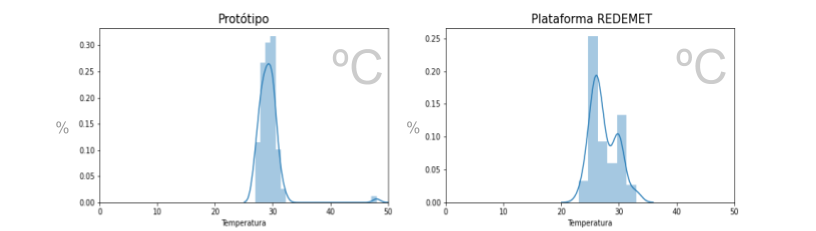
\includegraphics [scale = 0.5] {Figuras/dist_temp.png}
    \legend{Fonte: Gráfico elaborado pelo autor}
    \label{fig:dist_temperatura}
\end{figure}

É possível notar a presença de outliers nas medições feitas pelo protótipo. Facilmente observado no gráfico \ref{fig:box_temp}

\begin{figure} [!h]
    \centering
    \caption{Box Plot Temperatura}    
    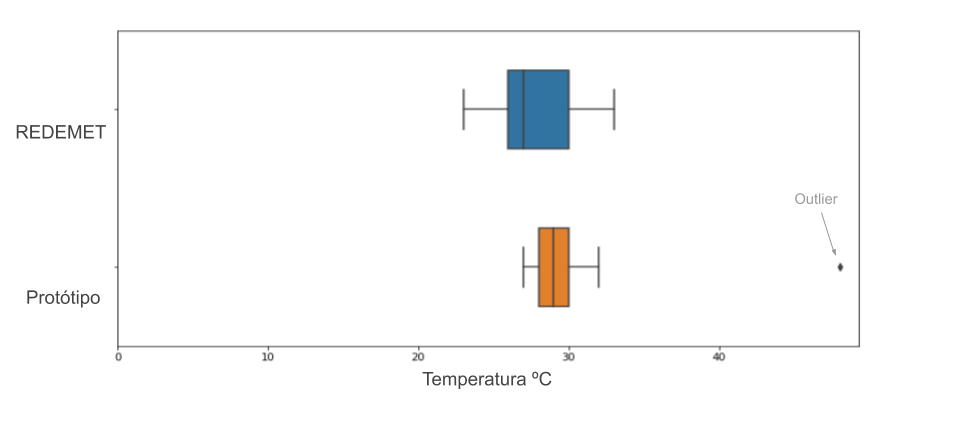
\includegraphics [scale = 0.45] {Figuras/box_temp.png}
    \legend{Fonte: Gráfico elaborado pelo autor}
    \label{fig:box_temp}
\end{figure}

Além de outliers é possível ver que a mediana das temperaturas coletadas pelo protótipo foi maior que a da plataforma REDEMET e que o menor valor de temperatura foi registrado na amostra da REDEMET. É o maior valor de temperatura foi registrado na amostra do protótipo justamente o outlier. Para confirmar essas observações e possível ver as estatísticas descritivas na tabela \ref{tab:est_desc_temp_prot}.

\begin{table}[!h]
\centering
\begin{tabular}{l|c|c|}
\cline{2-3}
                                                & \multicolumn{1}{l|}{\textbf{Temperatura REDEMET}} & \textbf{Temperatura Protótipo} \\ \hline
\multicolumn{1}{|l|}{Quantidade de Observações} & 90                                                & 90                             \\ \hline
\multicolumn{1}{|l|}{Média}                     & 27.37                                             & 29.30                          \\ \hline
\multicolumn{1}{|l|}{Desvio Padrão}             & 2.27                                              & 2.33                           \\ \hline
\multicolumn{1}{|l|}{Valor Mínimo}              & 23                                                & 27                             \\ \hline
\multicolumn{1}{|l|}{Valor Máximo}              & 33                                                & 48                             \\ \hline
\end{tabular}
\caption{Dados estatísticos variável temperatura}
\label{tab:est_desc_temp_prot}
\end{table}

\setlength\parindent{2em}
Aplicando o teste de distribuições o resultado foi que as amostras não são seguem o padrão da distribuição normal. Nesse caso será aplicado o cálculo estatístico de Wilcoxon, que deu como resultado que a hipótese H0 pode ser rejeitada com o pvalor de $4e-11$ um número muito próximo de zero. Nesse caso podemos concluir que para um nível de significância de 5\% as médias das temperaturas coletas pelo protótipo e pela plataforma REDEMET não são iguais.


\subsection{Análise da variável de pressão}

Na distribuição da variável de pressão podemos observar que ela foi mais uniforme e tivemos pouca diferença entre as amostras. Conforme gráfico \ref{fig:dist_pressao}

\begin{figure} [!h]
    \centering
    \caption{Distribuição da variável pressão}    
    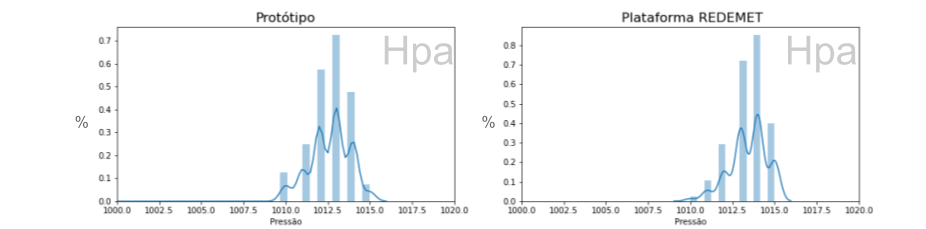
\includegraphics [scale = 0.5] {Figuras/dist_pressao.png}
    \label{fig:dist_pressao}
\end{figure}

Pelo gráfico \ref{fig:box_plot_pressao} é possível destacar a presença de outliers nas amostras. Visualmente as amostras têm resultados bem similares a diferença pode ser na questão de calibração do sensor. Nesse gráfico não é da para ver a mediana dos valores possivelmente foi igual algum intervalo interquartil do gráfico.

\begin{figure} [!h]
    \centering
    \caption{Box Plot Pressão}    
    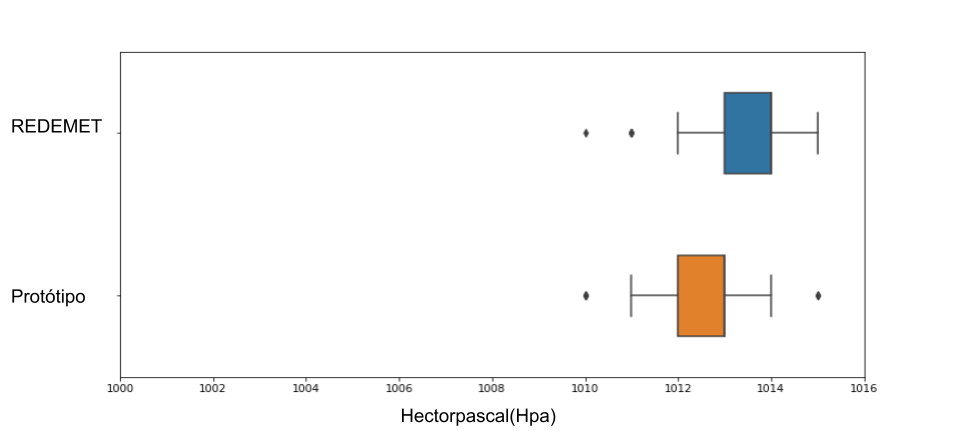
\includegraphics [scale = 0.45] {Figuras/box_plot_pressao.png}
    \label{fig:box_plot_pressao}
\end{figure}

Com as estatísticas descritivas da variável de pressão merece destaque o valor máximo que foi o mesmo para às duas amostras. O valor mínimo do protótipo é um outlier tivemos médias bem similares é um desvio padrão muito baixo na amostra da plataforma REDEMET. Conforme tabela \ref{tab:est_desc_pressao_prot}

\begin{table}[!h]
\centering
\begin{tabular}{l|c|c|}
\cline{2-3}
                                                & \multicolumn{1}{l|}{\textbf{Pressão REDEMET}} & \textbf{Pressão Protótipo} \\ \hline
\multicolumn{1}{|l|}{Quantidade de Observações} & 90                                            & 90                         \\ \hline
\multicolumn{1}{|l|}{Média}                     & 1013.44                                       & 1012.43                    \\ \hline
\multicolumn{1}{|l|}{Desvio Padrão}             & 1.11                                          & 2.2                        \\ \hline
\multicolumn{1}{|l|}{Valor Mínimo}              & 1010                                          & 995                        \\ \hline
\multicolumn{1}{|l|}{Valor Máximo}              & 1015                                          & 1015                       \\ \hline
\end{tabular}
\caption{Dados estatísticos variável pressão}
\label{tab:est_desc_pressao_prot}
\end{table}

O resultado do teste de normalidade foi favorável apenas para a amostra da plataforma REDEMET enquanto os dados do protótipo não se encaixaram em uma distribuição normal. Nesse caso será utilizado o cálculo estatístico de Wilcoxon que teve como resultado a rejeição da hipótese H0 com o pvalor muito baixo $1.73e-14$. Nesse caso podemos concluir que para um nível de significância de 5\% as médias das amostras coletas para a variável pressão do protótipo e da plataforma REDEMET não são iguais.

\subsection{Análise da variável de umidade}

As amostras da distribuição da variável de umidade são bem similares com poucas variações. Conforme gráfico \ref{fig:dist_umidade}. Visualmente pelo gráfico podemos notar que as destruições não seguem características de uma distribuição normal. Nenhum percentual de umidade foi registrado abaixo de 40\%. A maior parte das medições em ambas as amostras se concentrou próximas de 80\%.

\newpage

\begin{figure} [!h]
    \centering
    \caption{Distribuição da variável Umidade}
    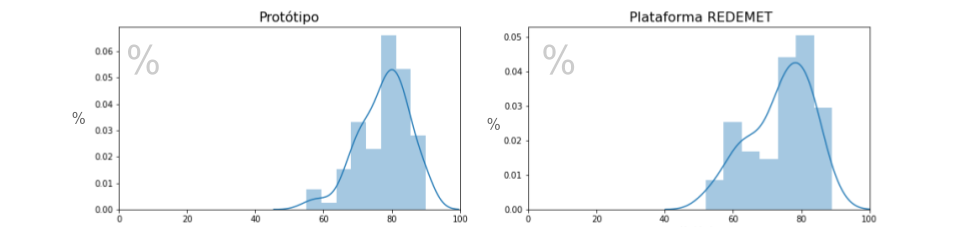
\includegraphics [scale = 0.5] {Figuras/dist_umidade.png}
    \label{fig:dist_umidade}
\end{figure}

Pelo gráfico \ref{fig:box_plot_umidade} podemos ver apenas um outlier na amostra do protótipo. A amostra do REDEMET tem mais variações nas medições do que a do protótipo. A mediana da amostra do protótipo é maior que a da amostra REDEMET. O maior valor de umidade foi registrado pela amostra do protótipo. O menor valor de umidade foi registrado pela plataforma REDEMET.

\begin{figure} [!h]
    \centering
    \caption{Box Plot Umidade}
    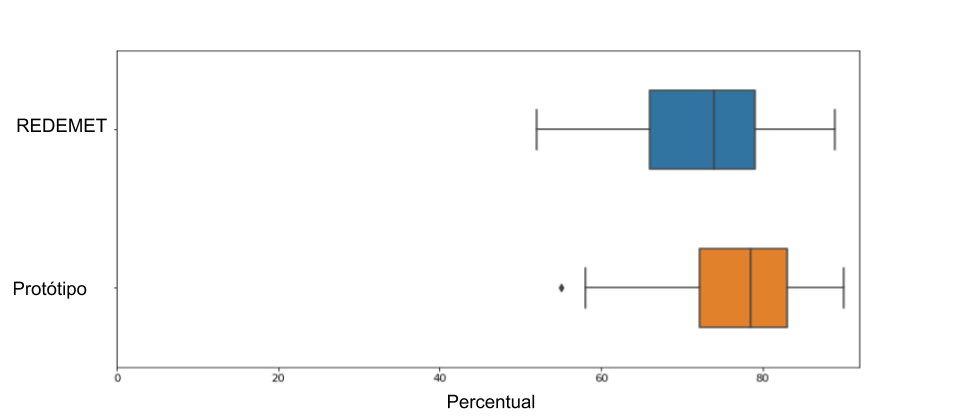
\includegraphics [scale = 0.5] {Figuras/box_plot_umidade.png}
    \label{fig:box_plot_umidade}
\end{figure}

Pela tabela \ref{tab:est_desc_umidade_prot} de dados estatísticos descritivos  podemos confirmar as observações feitas no gráfico. Podemos perceber um desvio padrão muito elevado nas amostras.

\begin{table}[!h]
\centering
\begin{tabular}{l|c|c|}
\cline{2-3}
                                                & \multicolumn{1}{l|}{\textbf{Umidade REDEMET}} & \textbf{Umidade Protótipo} \\ \hline
\multicolumn{1}{|l|}{Quantidade de Observações} & 90                                            & 90                         \\ \hline
\multicolumn{1}{|l|}{Média}                     & 73.84                                         & 77.67                      \\ \hline
\multicolumn{1}{|l|}{Desvio Padrão}             & 9.16                                          & 7.40                       \\ \hline
\multicolumn{1}{|l|}{Valor Mínimo}              & 52                                            & 55                         \\ \hline
\multicolumn{1}{|l|}{Valor Máximo}              & 89                                            & 90                         \\ \hline
\end{tabular}
\caption{Dados estatísticos variável umidade}
\label{tab:est_desc_umidade_prot}
\end{table}

Aplicando o teste de normalidade nas distribuições apenas a amostra da REDEMET pode ser classificada como normal. Aplicando o teste de Wilcoxon tivemos como resultado a rejeição da hipótese H0 com o pvalor muito baixo $2.94e-11$. Nesse caso podemos concluir que para um nível de significância de 5\% as médias das amostras coletas para a variável umidade não são iguais.

\subsection{Análise da variável direção do vento}

A distribuição das amostras para essa variável foi bem distinta. Como podemos observar no gráfico de distribuição. A concentração das medições ficou similar nas amostras com valores próximos a 100 graus.

\begin{figure} [!h]
    \centering
    \caption{Distribuição da variável direção do vento}    
    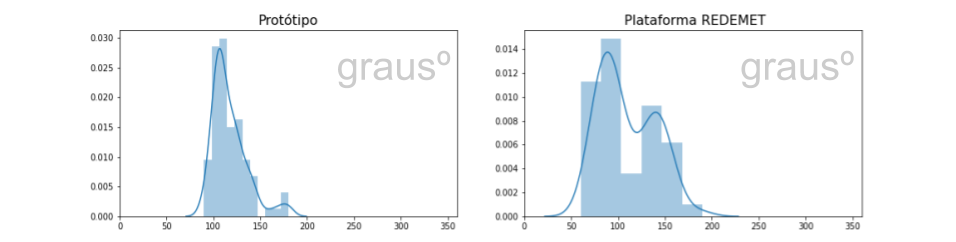
\includegraphics [scale = 0.5] {Figuras/dist_dirvento.png}
    \label{fig:dist_dirvento}
\end{figure}

No gráfico \ref{fig:box_plot_dirvento} existe a presença de outliers na amostra do protótipo. A mediana da amostra do protótipo foi superior a da REDEMET. Fica mais evidente a grande variação dos valores na amostra da plataforma REDEMET. 

\begin{figure} [!h]
    \centering
    \caption{Box Plot Direção do Vento}
    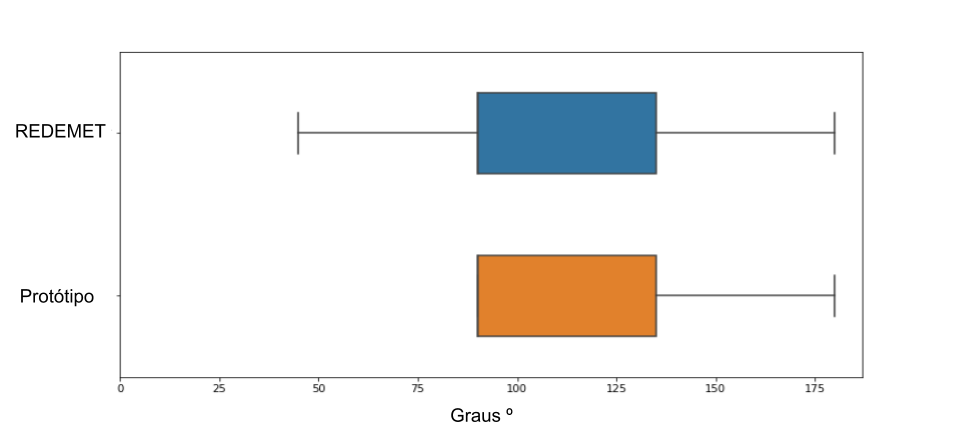
\includegraphics [scale = 0.5] {Figuras/box_plot_dirvento.png}
    \label{fig:box_plot_dirvento}
\end{figure}

Os valores de mensuração do sensor do protótipo são limitados aos pontos cardeais e colaterais o que dá no total oito valores (0º, 45º, 90º, 135º, 180º, 225º, 270º e 315º) possíveis enquanto os dados coletados na amostra REDEMET mostram maiores variações. As estatísticas descritivas mostram um grande desvio padrão na variável a média dos valores ficou bem próxima. Os valores máximo e mínimo mostram o problema de precisão do sensor do protótipo que não conseguiria medir o valor 60 nem 190.

\begin{table}[]
\centering
\begin{tabular}{l|c|c|}
\cline{2-3}
                                                & \multicolumn{1}{l|}{\textbf{Umidade REDEMET}} & \textbf{Umidade Protótipo} \\ \hline
\multicolumn{1}{|l|}{Quantidade de Observações} & 90                                            & 90                         \\ \hline
\multicolumn{1}{|l|}{Média}                     & 109.66                                        & 117.24                     \\ \hline
\multicolumn{1}{|l|}{Desvio Padrão}             & 29.65                                         & 18.82                      \\ \hline
\multicolumn{1}{|l|}{Valor Mínimo}              & 60                                            & 90                         \\ \hline
\multicolumn{1}{|l|}{Valor Máximo}              & 190                                           & 180                        \\ \hline
\end{tabular}
\caption{Dados estatísticos variável direção do vento}
\label{tab:est_desc_dirvento_prot}
\end{table}

No teste de normalidade o resultado foi que ambas as amostras não seguem o padrão da distribuição normal. Na aplicação do teste de Wilcoxon tivemos como resultado do pvalor de 0,00079 bem inferior ao nível de significância. Nesse caso podemos concluir que as médias das amostras do protótipo e da plataforma REDEMET não são iguais para um nível de significância de 5\%.

\subsection{Análise da variável velocidade do vento}

As mensurações de velocidade vento pelo protótipo não foram bem sucedidas houve a queima do sensor que conta as rotações das pás, o reed switch, durante os experimentos desse modo conforme o gráfico \ref{fig:dist_velvento} demonstra que a amostra do protótipo foram bem pequenas. 

\begin{figure} [!h]
    \centering
    \caption{Distribuição da variável direção do vento}    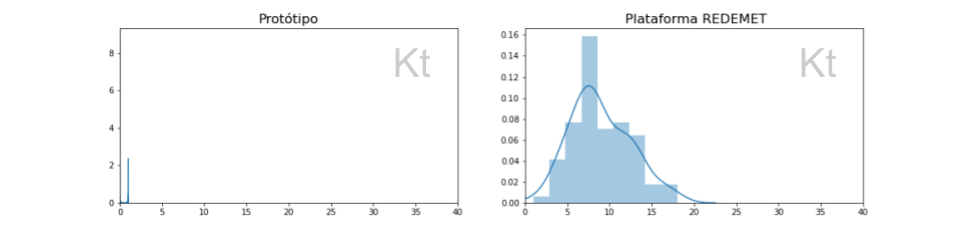
\includegraphics [scale = 0.5] {Figuras/dist_velvento.png}
    \label{fig:dist_velvento}
\end{figure}


Para confirmar que as mensurações de velocidade do vento não foram suficientes pelo protótipo no gráfico \ref{fig:box_plot_velvento} notamos que a amostra foi considerada como um outlier. Enquanto a amostra da plataforma REDEMET se mostrou bem distribuída e sem a presença de outliers. Com a média entre os valores de 25\% a 50\% da amostra. É com valor máximo superior a 17,5 kt e valor mínimo próximo à média dos valores coletados pelo protótipo.

\begin{figure} [!h]
    \centering
    \caption{Box Plot Velocidade do Vento}
    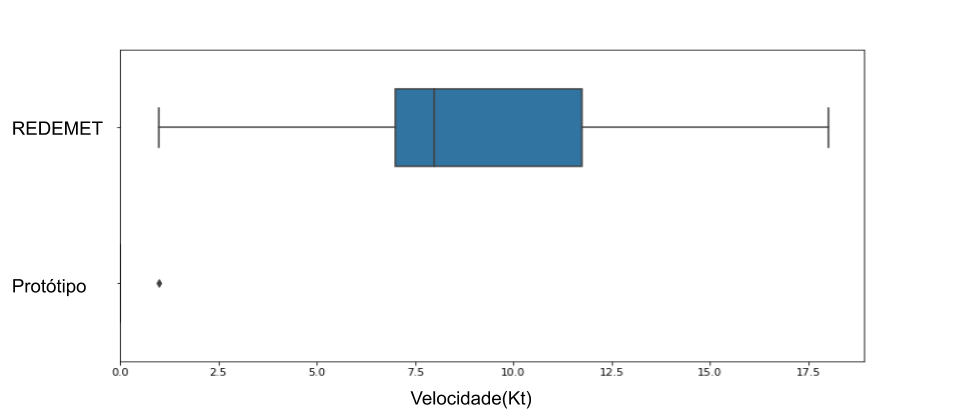
\includegraphics [scale = 0.5] {Figuras/box_plot_vento.png}
    \label{fig:box_plot_velvento}
\end{figure}

Observando os valores das estatísticas descritivas na tabela \ref{tab:est_desc_velvento_prot} se confirma as observações feitas na análise do gráfico de box plot.

\begin{table}[]
\centering
\begin{tabular}{l|c|c|}
\cline{2-3}
                                                & \multicolumn{1}{l|}{\textbf{Umidade REDEMET}} & \textbf{Umidade Protótipo} \\ \hline
\multicolumn{1}{|l|}{Quantidade de Observações} & 90                                            & 90                         \\ \hline
\multicolumn{1}{|l|}{Média}                     & 8.94                                          & 0.011                      \\ \hline
\multicolumn{1}{|l|}{Desvio Padrão}             & 3.56                                          & 0.01                       \\ \hline
\multicolumn{1}{|l|}{Valor Mínimo}              & 1                                             & 0                          \\ \hline
\multicolumn{1}{|l|}{Valor Máximo}              & 18                                            & 1                          \\ \hline
\end{tabular}
\caption{Dados estatísticos variável velocidade do vento}
\label{tab:est_desc_velvento_prot}
\end{table}

É evidente que a distribuição do protótipo não é normal aplicando o teste de normalidade essa observação se confirmou e a distribuição da REDEMET foi classificada como normal. Foi aplicado o teste de Wilcoxon mesmo já sabendo que o resultado seria rejeição que se confirmou com um pvalor de 0,0014. É possível concluir que as médias das amostras do protótipo e da plataforma REDEMET não são iguais para um nível de significância de 5\%.

